\section{Subject Decisions}\label{app:subtasks}

\pmt{I'm not going to futz with the sections right now, but I would make section 4 Subject Decisions, then have various subsections}
\pmst{We begin with a brief overview of subject behavior in the different tasks. }

%XXXX NEED TO REWRITE HERE XXXX}

Overall, we find that subject behavior across our tasks is largely ``sensible," i.e., subjects respond to increases in risk by protecting more, but deviates from the risk-neutral theoretical benchmark.  Below we investigate several standard possible explanations, including risk preferences and failures of Bayesian updating, before exploring how the characteristics of the signal influences protection decisions, beliefs, and WTP.

We follow that discussion with a regression analysis to explain subjects' WTP for signals of different qualities. Our regression results suggest that subjects' WTP deviated from those of a risk-neutral utility maximizing subject which was driven by their failure to fully account for signal quality when calculating their WTP. Furthermore, we find that these deviations remained after controlling for risk aversion or subjects' ability to perform Bayesian updating. 

%The final subsection explored theories that are consistent with these observed behaviors.



%\subsection{Overview: Are Subjects Bounded Rational?}
\subsection{Blind Protection}



\pmst{\textbf{Blind Protection.}}\pmst{Subjects' responses in the BP task are generally consistent with the expected utility framework.} Figure~\ref{fig:ProtResponse} plots the probability of protection decision against \pmst{prior}posterior probability of a black ball for the BP task, where the posterior is equivalent to the prior, and the IP task. On aggregate, subjects protect more with a higher probability of a negative outcome: only 13\% subjects protect when the probability of a black ball is 10\% in contrast to 70\% protecting when the probability is 30\%. 
%Moreover, the majority of subjects (54\%) have a probability threshold above which they always protect. About 30\% of subjects make at least one switch in which they protect for probability $P_1$ and do not protect for at least one probability $P_2>P_1$. 

At the individual level, BP responses are also largely sensible but  indicate significant heterogeneity in terms of risk aversion. For approximately 70\% of subjects (X/Y), the probability of choosing protection increases monotonically in posterior probability. The remaining 30\% make at least one switch from protecting to not protecting and back, which is inconsistent with EU maximization. Among these switchers, however, 83\% (24/39) skip only a single increment of the presented probability scale, suggesting an inattention error.\footnote{For comparison, this reference on the Holt and Laury (2002) instrument suggests the XX\% (YY\%) of subjects switch at least (at most) once.}  Risk-neutral subjects maximize their expected utility by protecting whenever the prior probability exceeds 0.25, which is the ratio of the protection cost (\$5) to the potential loss (\$20). In contrast, many of our subjects start protecting for lower probabilities of 0.1 or 0.2 indicating strict risk aversion. As a point of reference, switching at the probability 0.1 corresponds to CRRA risk aversion of $\theta=2$, while switching at 0.2 corresponds to $\theta=0.573$ (see \ref{ra_table} in Appendix).  \aut{I need to review the literature here to compare.} A smaller group of subjects makes choices consistent with risk loving by never protecting or protecting for the probability of 0.3. We use the total number of protection choices as a measure of subjects' risk aversion, but following Holt and Laury (2002) exclude subjects switching more than once. Most of our results do not condition on risk aversion and hence are not affected by this calculation. \pmt{I don't understand exactly what you mean by using the total to ``calculate" risk preferences.  In HL, the total corresponds to a range for the parameter of a CRRA utility function, but I think we are just using the total as a relative metric in our sample?  Also, we probably need to make sure that everything doesn't go totally bananas if we include the multiple switchers, then offer in a footnote to send those results to anyone who cares.}

\subsection{Informed Protection}
%\bigskip\noindent\textbf{Informed Protection/Response to Signal.}\ \ \
Protection decisions are also positively correlated across tasks for a given individual.
Subjects receive more information in the IP task than in the BP task, though using that information requires that subjects engage in Bayesian updating.  Figure~\ref{fig:ProtResponse} shows that, consistent with their behavior in the BP task, the share of subjects protecting in the IP task is increasing in the posterior probabilities. Roughly 28\% of subjects break monotonicity in their protection responses with respect to posterior probabilities\footnote{ They do not protect for some treatments with posterior probability $P$ while protecting for a posterior probabilty $P'<P$.} which roughly equals the percentage of non-monotonic responses for the BP task. At the individual level, we also observe that the total number of times subjects choose protection in the BP task significantly correlates with their likelihood to protect in the IP task conditional on posteriors, but this explains only a very small part ($<$1\%) of variation in the IP decisions\footnote{We use a LPM to estimate this relationship, and while the coefficient on the total number of protection choices is significant at 99\%, $R^2$ increases from 0.295 to 0.3.} 

Subjects' responses in the first two tasks suggest that conditional on the true probabilities, subjects protected more in the IP task compared to the BP task at low probabilities, \aut{even though the difference is not statistically significant}\pmt{What is the test? Proportion of protection decisions for probabilities less than X or something?}. These choices suggest that subjects' updated beliefs overshot the true posterior at low probabilities.  Unfortunately, we cannot compare their decisions for higher probabilities because we do not present choices with higher prior in the BP task.

%%%%%%%%%%%%%%%%%%%%%%%%%%%%%%%%%%%%%%%%%%%%%%%%%%%%%%%%%%%%%%%%%%%%%%%%%%%%%%%%%%%%%%%%%%%%%%%%%%%%%%%%%%%%%%%%%%%

\begin{figure}[H]
\centering
\caption{Average Protection Response} \label{fig:ProtResponse}
\begin{subfigure}[t]{.45\textwidth}
  \centering
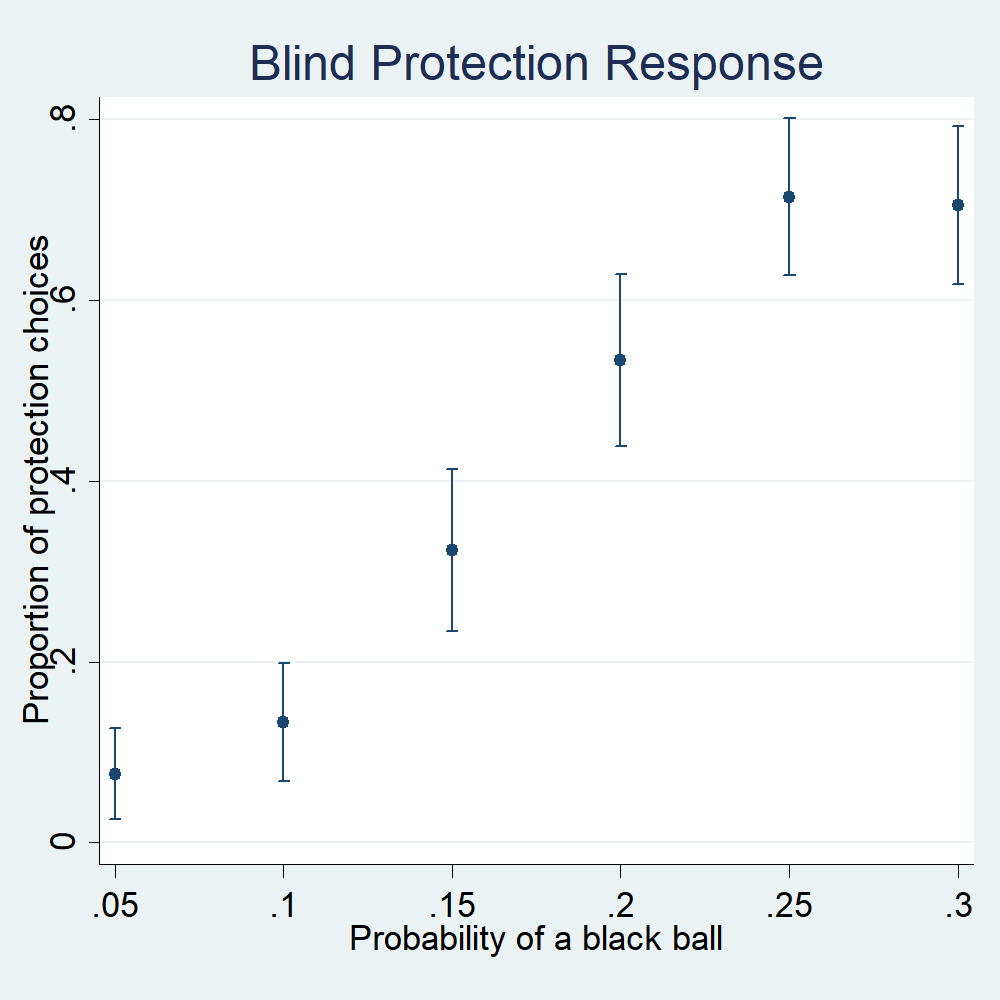
\includegraphics[width=\textwidth]{Graphs/blind_prot_sta.png}
\end{subfigure}
\begin{subfigure}[t]{.45\textwidth}
  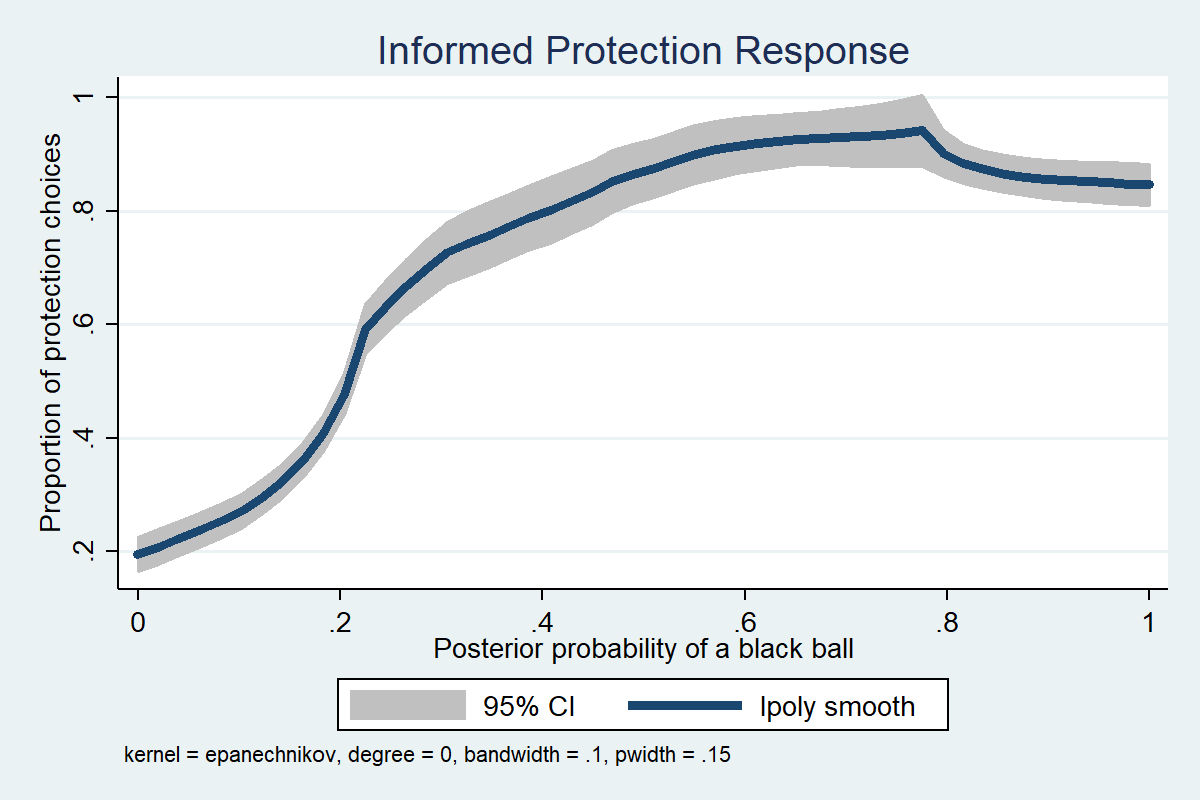
\includegraphics[width=\textwidth]{Graphs/ip_response_lpoly.png}
\end{subfigure}
%\begin{subfigure}[t]{.48\textwidth}
  %\centering
  %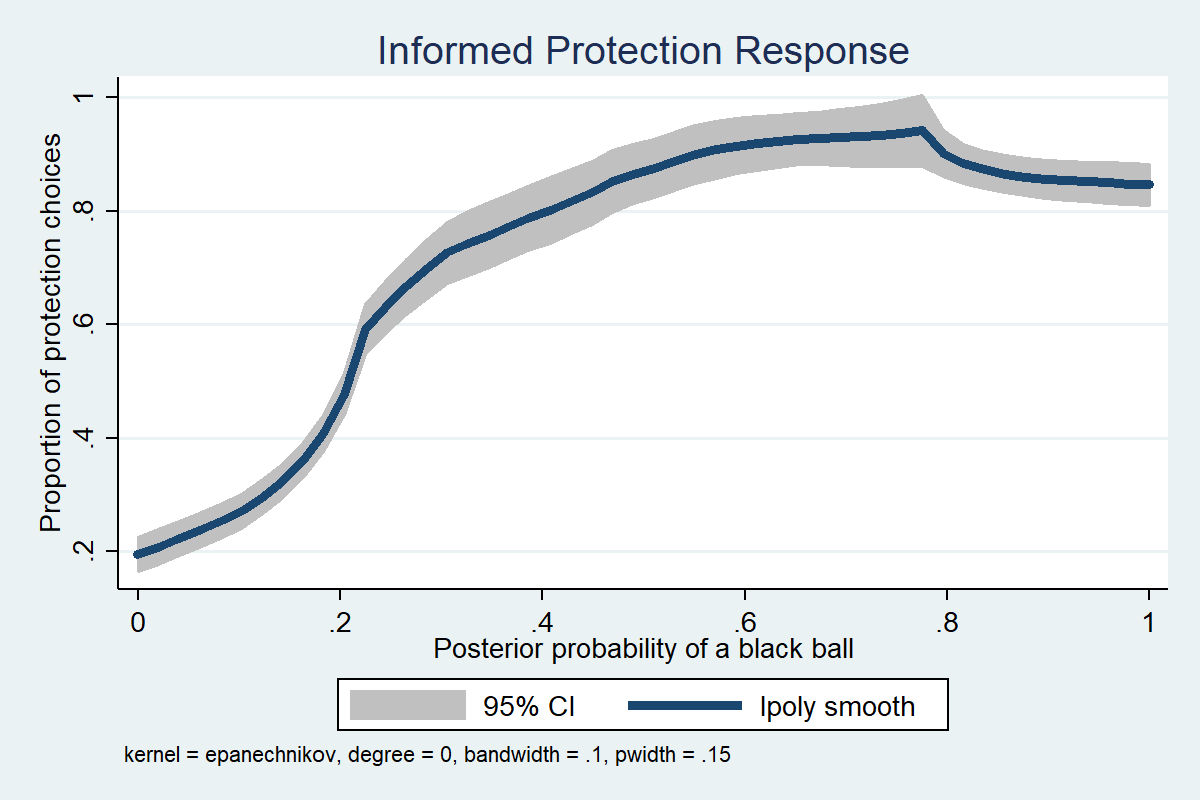
\includegraphics[width=\textwidth]{Graphs/ip_response_lpoly.png}
%
%\end{subfigure}
\end{figure}
\pmt{Eventually we need to add notes to the figures}
%%%%%%%%%%%%%%%%%%%%%%%%%%%%%%%%%%%%%%%%%%%%%%%%%%%%%%%%%%%%%%%%%%%%%%%%%%%%%%%%%%%%%%%%%%%%%%%%%%%%%%%%%%%%%%%%%%%

%\bigskip\noindent\textbf{Belief Elicitation.}\ \ \ 
\subsection{Belief Elicitation}
While the IP task gives us a sense for how subjects utilize signals in making protection decisions, we observe only whether or not they choose to protect, which conflates preferences with potential errors in updating posteriors.  The BP task gives provides insight into subjects' risk preferences, while the BE task allows us to better understand to what extent updating errors influence decisions.  

We define updating errors as the difference between the posterior and subjects' elicited belief on the posterior probability of a black ball for a given signal.  We plot the distribution of the updating errors in the left hand column of Figure~\ref{fig:BeliefUpdate}, while the right hand column provides a scatter plot of the elicited beliefs against the true posterior with a fitted line.\pmt{I would prefer to take the r-squared out of this figure and put it in the table note with the correlations for each panel}\aut{Duly noted, will be incorporated.}.
%Since subjects were only given signal characteristics and not true posteriors, their IP responses reflect, inter alia, their ability to infer the true posteriors from signal characteristics. (I'm not sure I like my sentence better)
Panel A of Figure~\ref{fig:BeliefUpdate} uses all elicited beliefs and suggests that, while errors occur, beliefs are still sensible. The distribution of updating errors is centered at 0, with roughly one-half (51\%) concentrated within +/- 0.1 interval around zero. Overall, the correlation between the elicited beliefs and the true posteriors was 0.653.  

Using all the observations, however, obscures an important distinction: in many cases the ball color is completely certain based on priors and signals and so the updating should be trivial.  Panel B of Figure~\ref{fig:BeliefUpdate} includes only those 44\% beliefs elicited for an uncertain posterior. The median error is now -0.12, with with 90\% of errors between -0.48 and 0.3, suggesting that subjects tend to overestimate the likelihood of adverse events for uncertain posteriors, \pmt{which is consistent with what we see in Figure~\ref{fig:ProtResponse}}. The correlation between beliefs and posteriors in this subset of observations is only 0.571.  Panel C of Figure~\ref{fig:BeliefUpdate} plots the distribution of updating errors with certain posteriors, which includes: (i) treatments with all-honest gremlins; and (ii) treatments with obviously irrelevant dishonest gremlins (e.g., a group with honest and white-eyed gremlins with a hint that the ball is black --- or vice versa). Reassuringly, 69\% of reported beliefs are correct, but subjects still err in about 30\% of cases. About half of these errors involve reporting a probability of between one and zero, with the other half reporting a probability of one when it should have been zero. \aut{There is little evidence of these drastic errors (0 instead of 1) being strongly correlated with randomness in other treatments.} \pmt{It depends a bit.  Are some guys doing everything right here and others doing everything wrong?  Is there any relationship between errors here and inconsistencies in BP or a lower correlation between BP and IP tasks?} 

Overall, the pattern of belief updating is consistent with previous literature which finds that while humans usually update beliefs in a correct direction, they tend to underreact both to priors and the signals. The effect of underweighting priors, first noted in the psychology literature \citep*{phillips_conservatism_1966-1, tversky_belief_1971, kahneman_subjective_1972}, and is known under the names of representativeness bias or base rate neglect. Subjects sensitivity both to priors and signals is easy to measure through estimating the following equation ((first introduced by \citet{grether_bayes_1980}) which links the posterior probabilities $\mu(B|S)$ of the state $B$ conditional on signal $S$ with the prior log-odds $\log\left({P(S|B) \over P(S|W)}\right)$ of the signal and signal log-odds $\log \left({P(B)\over P(W)}\right)$: 
\begin{equation}
\log\left({\mu(B|S) \over 1-\mu(B|S)}\right)=\alpha \log\left({P(S|B) \over P(S|W)}\right)+\beta \log \left({P(B)\over P(W)}\right)
\end{equation}

Coefficients $\alpha$ and $\beta$ should equal one if subjects perfectly follow Bayesian updating. Our estimates of these parameters are significantly below one with $\hat \alpha=0.43$ $\hat \beta=0.25$ (see Column 1 in \ref{belief_decomposition}). This is consistent with the meta-analysis in \citet{benjamin_chapter_2019} which calculates the average $\hat \alpha$ estimate to be around 0.22 (0.4 for incentivized studies only) and the average $\hat \beta$ to be 0.6 (0.43 for incentivized) for studies presenting signals simultaneously (consistent with this study)\footnote{The common name for this kinds of experiments is \textit{bookbag-and-poker-chip experiments}}. Hence our subjects also demonstrate both the base-rate neglect and the signals underweighting. These effects lower the correlation between posteriors and reported beliefs and reduce sensitivity of beliefs to signal characteristics.  


%%%%%%%%%%%%%%%%%%%%%%%%%%%%%%%%%%%%%%%%%%%%%%%%%%%%%%%%%%%%%%%%%%%%%%%%%%%%%%%%%%%%%%%%%%%%%%%%%%%%%%%%%%%%%%%%%%%

\begin{figure}[H]
	\centering
	\caption{Errors in Bayesian Updating} \label{fig:BeliefUpdate}
	\subcaptionbox{Error Distribution}{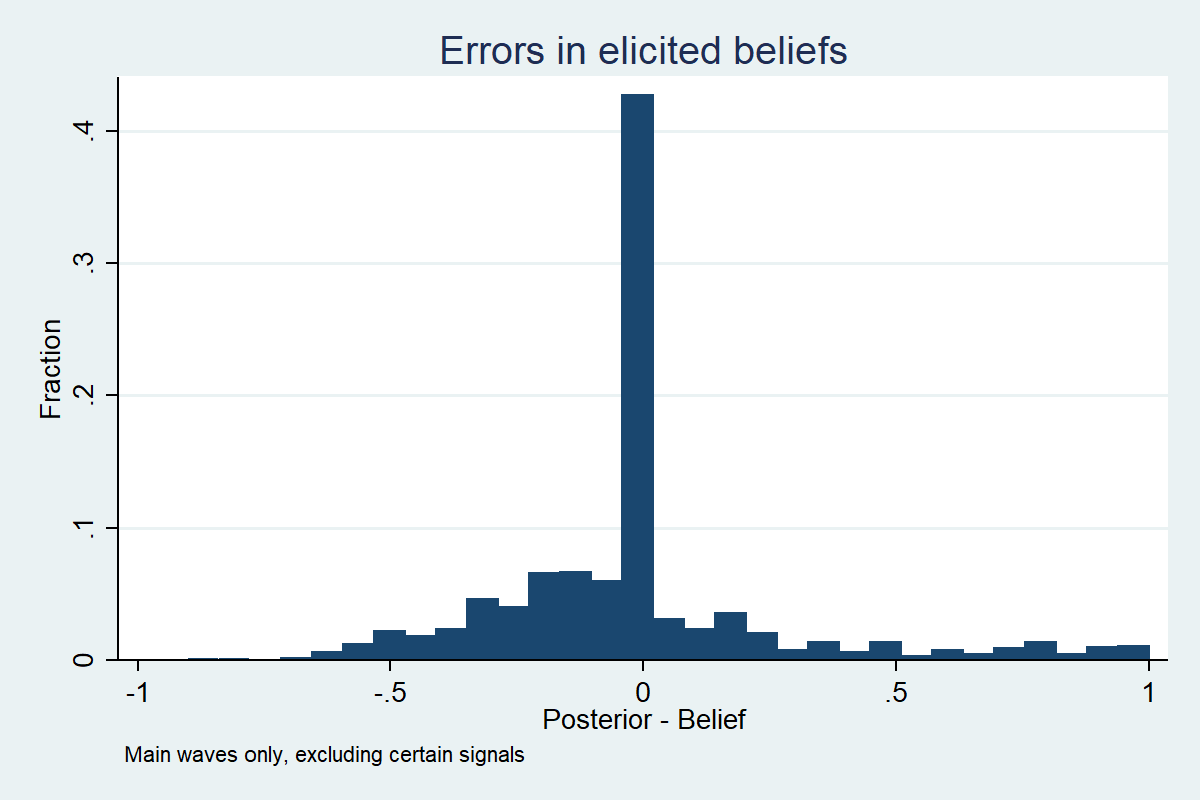
\includegraphics[width=.48\textwidth]{Graphs/hist_belief_error_s3.png}}
	\hfill
	\subcaptionbox{Error v. Posterior}{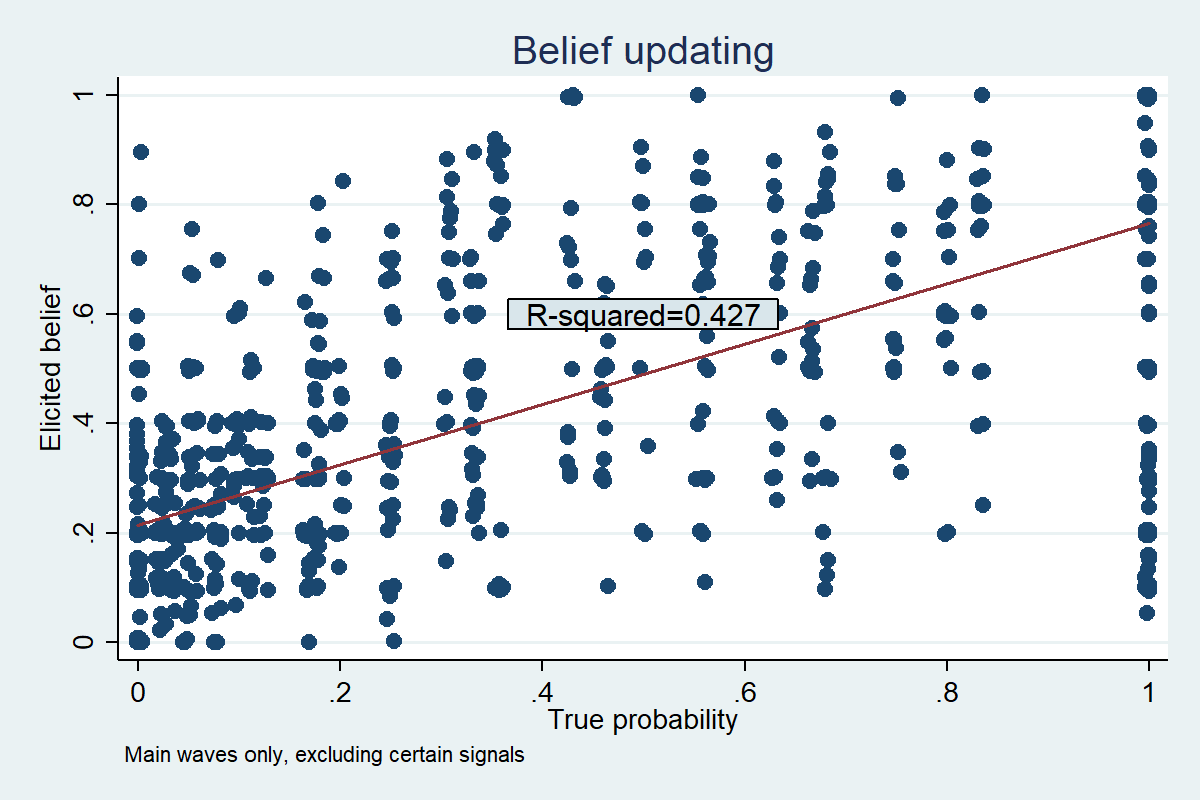
\includegraphics[width=.48\textwidth]{Graphs/updating_s3.png}}
	\hfill
	\subcaptionbox{Error Distribution, Uncertain Color}{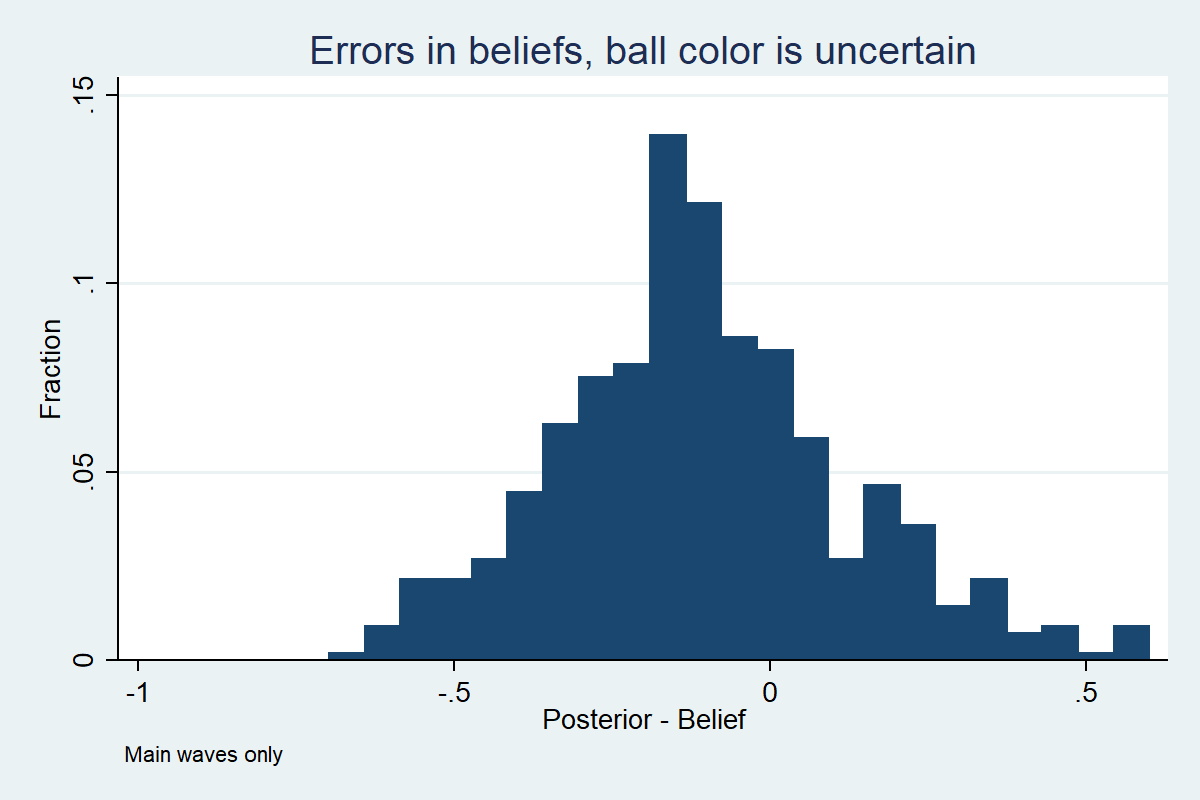
\includegraphics[width=.48\textwidth]{Graphs/hist_belief_error_s4.png}}
	\hfill
	\subcaptionbox{Error v. Posterior, Uncertain Color}{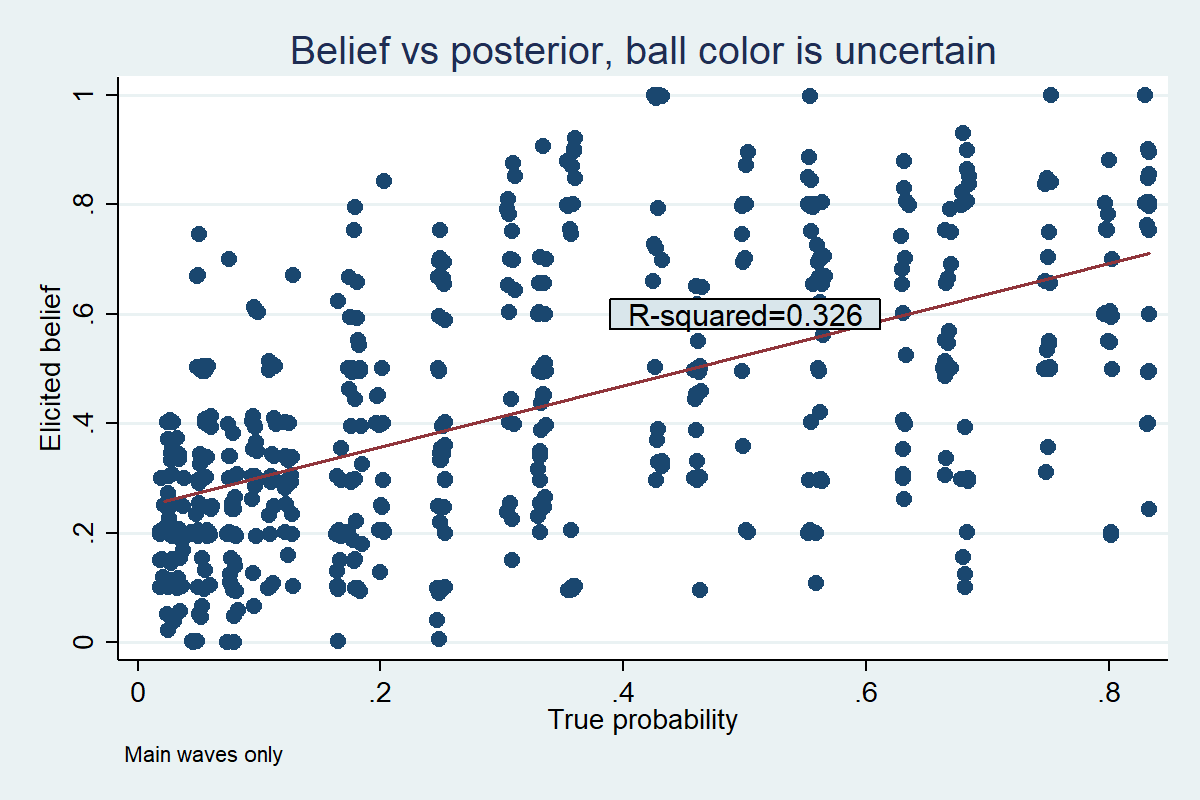
\includegraphics[width=.48\textwidth]{Graphs/updating_s4.png}}
	\hfill
	\subcaptionbox{Error Distribution, Certain Color}{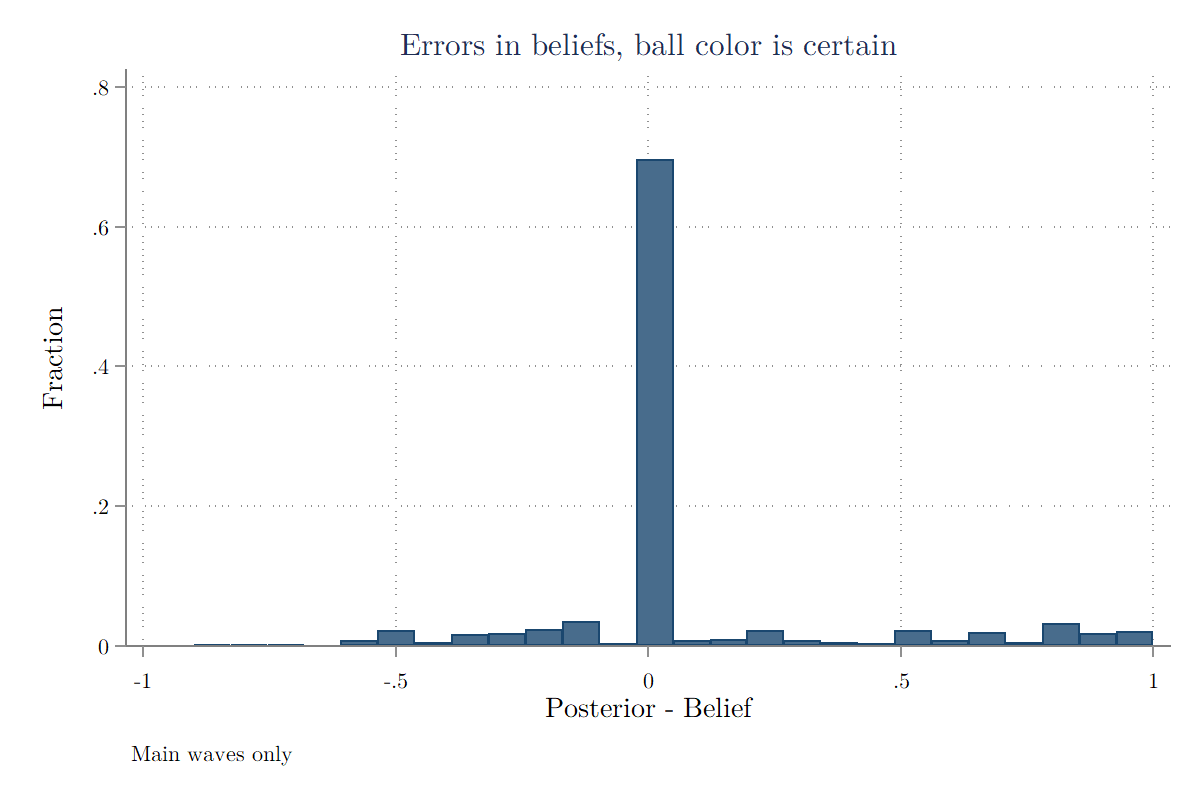
\includegraphics[width=.48\textwidth]{Graphs/hist_belief_error_s5.png}}
	\hfill
	\subcaptionbox{Error v. Posterior, Certain Color}{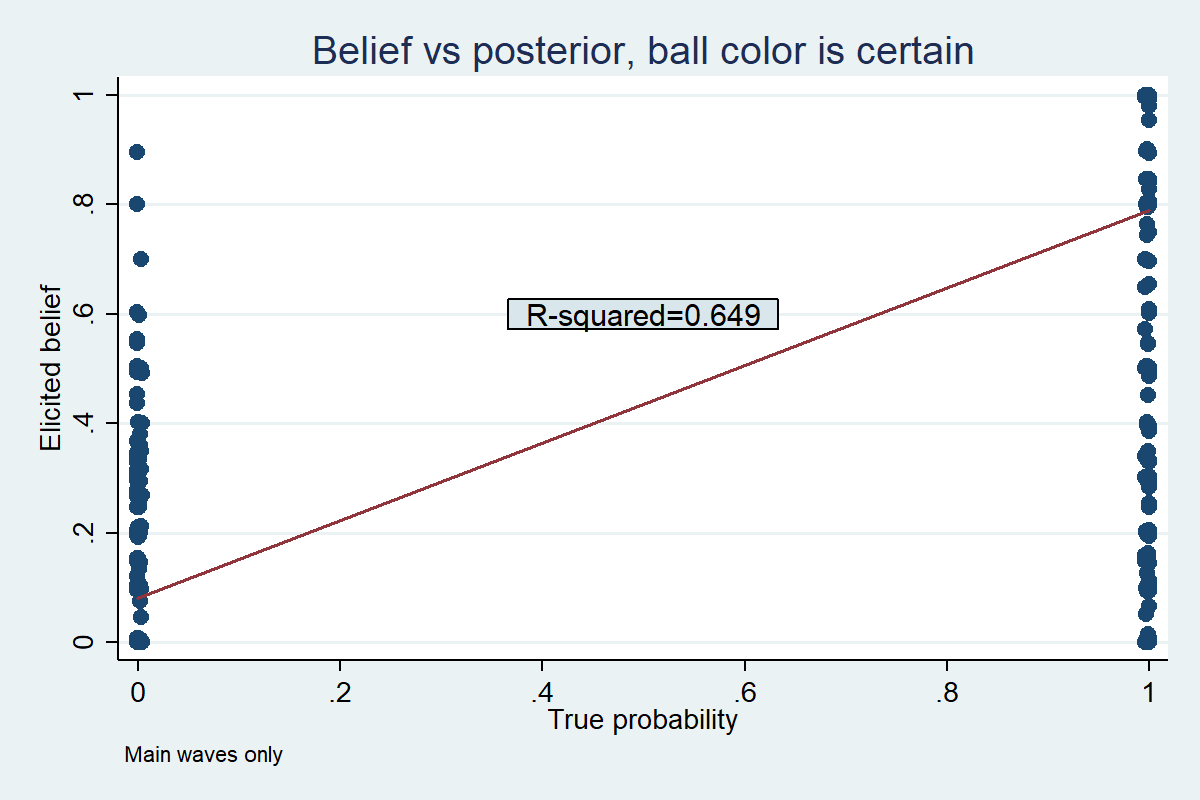
\includegraphics[width=.48\textwidth]{Graphs/updating_s5.png}}
	\hfill
\end{figure}
\clearpage

%%%%%%%%%%%%%%%%%%%%%%%%%%%%%%%%%%%%%%%%%%%%%%%%%%%%%%%%%%%%%%%%%%%%%%%%%%%%%%%%%%%%%%%%%%%%%%%%%%%%%%%%%%%%%%%%%%%

%\bigskip\noindent\textbf{Willingness-to-Pay Elicitation.}\ \ \ 
%\subsection{Willingness-to-Pay Elicitation}
%The BP, IP, and BE tasks allow us to discern how individuals use freely provided information to make protection decisions, but signals are not necessarily provided freely.  To better understand how subjects value the signals, we elicit their Willingness-to-Pay for signals of differing degrees of informativeness.  Figure XX plots the distributions of the theoretically optimal WTP\pmt{We should explain here where this comes from} (Panel A), the distribution of actual WTP (Panel B), and the distribution of the discrepancies between the theoretical and actual WTP that we observe.  WTP is bounded between \$0 and \$5, where the latter is because protection can be purchased for \$5 so if information were that valuable, an individual would just choose to protect.  \pmt{Placeholder for where we say something about my suggested Panels A and B.}  Reported WTP is centered around the theoretical WTP, suggesting that it is a useful benchmark. However, the variation is very substantial. Only 25\% of actual WTP are within \$0.50 if the theoretical one, and subjects overvalue the signal by at least \$1.5 in 22\% of cases and undervalue it  by at least \$1.5 in 19\% of cases. 
%
%\begin{figure}[H]\centering 
%\caption{Willingness-to-Pay Distribution} \label{fig:WTPhist}
%\subcaptionbox{Value Distribution}{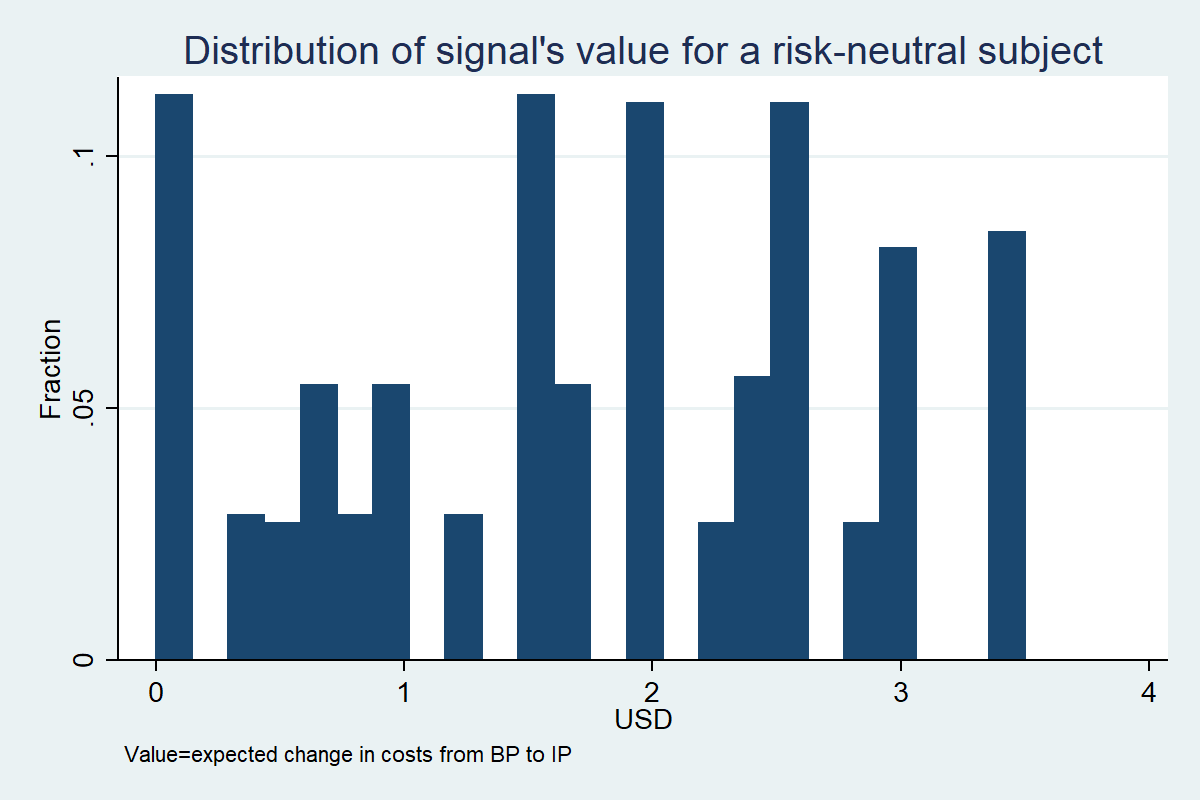
\includegraphics[scale=0.2]{Graphs/hist_value.png}}
	%\hfill
%\subcaptionbox{WTP distribution}{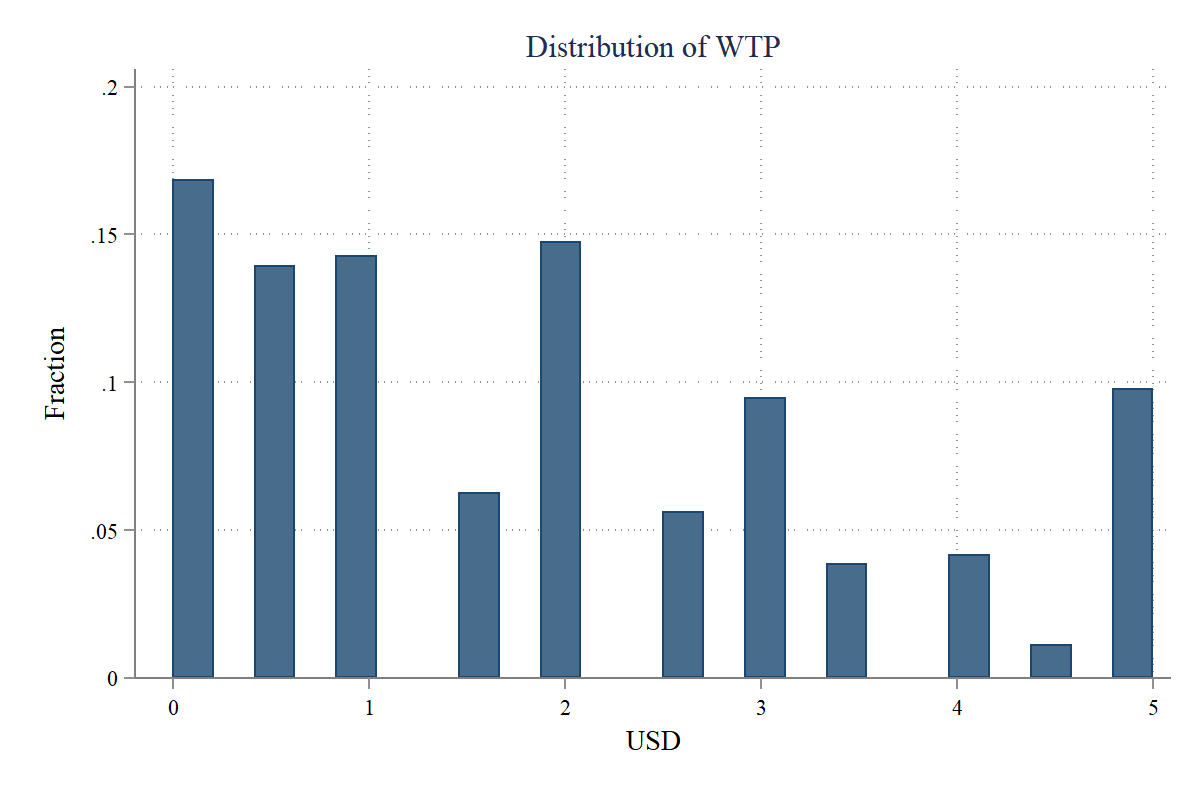
\includegraphics[scale=0.2]{Graphs/hist_WTP.png}}
	%\hfill
%\subcaptionbox{Discrepancy (WTP-Value)}{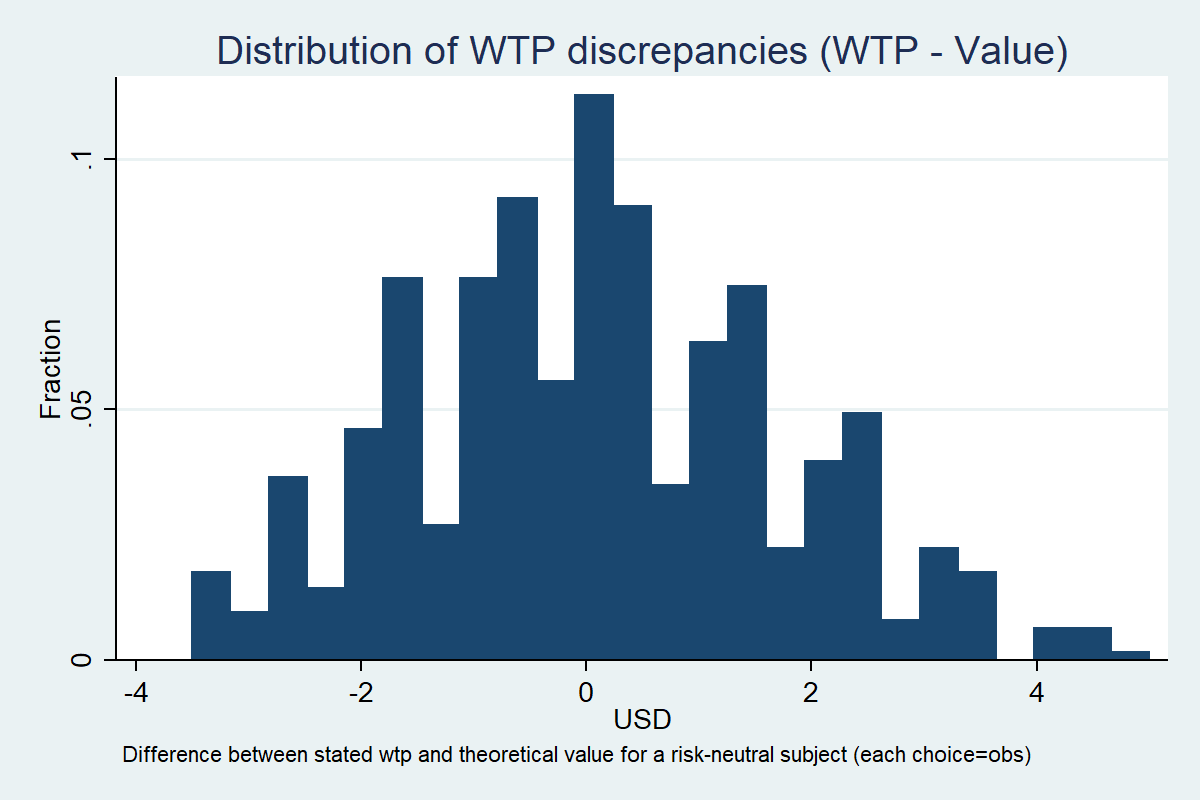
\includegraphics[scale=0.2]{Graphs/hist_WTP_discr1.png}}
	%\hfill
%\end{figure}
